% =====================================================================
% FINAL REPORT: MAP-RAG-Gym
% Compile with pdfLaTeX.
% =====================================================================

\documentclass[12pt,a4paper]{article}

\usepackage[utf8]{inputenc}
\usepackage[T5]{fontenc}
\usepackage[vietnamese,english]{babel}
\usepackage{times}
\usepackage[margin=2.5cm]{geometry}
\usepackage{setspace}
\setstretch{1.15}
\setlength{\parskip}{5pt}
\setlength{\parindent}{1.2cm}

\usepackage{graphicx}
\usepackage{amsmath,amssymb,amsfonts}
\usepackage{booktabs}
\usepackage{multirow}
\usepackage{array}
\usepackage{caption}
\usepackage{subcaption}
\usepackage{float}
\usepackage{enumitem}
\usepackage{hyperref}
\usepackage{xcolor}
\usepackage{titlesec}
\usepackage{fancyhdr}
\usepackage{algorithm}
\usepackage{algorithmic}
\usepackage{microtype}
\usepackage{url}
\usepackage{longtable}
\usepackage[numbers,sort&compress]{natbib}

\definecolor{mainblue}{RGB}{0,71,140}
\definecolor{notered}{RGB}{170,20,20}

\hypersetup{
    colorlinks=true,
    linkcolor=mainblue,
    citecolor=mainblue,
    urlcolor=mainblue
}

\titleformat{\section}{\large\bfseries\color{black}}{\thesection.}{0.5em}{}
\titleformat{\subsection}{\normalsize\bfseries\color{black}}{\thesubsection.}{0.5em}{}
\titleformat{\subsubsection}{\normalsize\itshape\bfseries\color{black}}{\thesubsubsection.}{0.5em}{}

\pagestyle{fancy}
\fancyhf{}
\lhead{MAP-RAG-Gym Final Report}
\rhead{\thepage}
\renewcommand{\headrulewidth}{0.4pt}
\setlength{\headheight}{15pt}

\newcommand{\vnote}[1]{{\selectlanguage{vietnamese}\noindent\textcolor{notered}{\textbf{Ghi chú:} #1}\selectlanguage{english}}}

\begin{document}

\begin{titlepage}
    \centering
    \vspace*{0.5cm}
    {\Large \textbf{UNIVERSITY / FACULTY / DEPARTMENT NAME}}\\[0.3cm]
    {\large \textbf{COURSE NAME}}\\[1.5cm]

    {\Huge \textbf{FINAL REPORT}}\\[0.7cm]
    {\LARGE \textbf{MAP-RAG-Gym: Adaptive Multi-Workflow Retrieval-Augmented Generation with Process-Level Evaluation}}\\[0.8cm]
    {\large \textit{A budget-aware system combining macro workflow routing and micro process criticism for knowledge-intensive question answering}}\\[1.5cm]

    \begin{tabular}{rl}
        \textbf{Instructor:} & Instructor full name \\
        \textbf{Course section:} & Class name / Course code \\
        \textbf{Group:} & Group name or group number \\
        \textbf{Submission date:} & dd/mm/yyyy \\
    \end{tabular}

    \vfill
    {\large \textbf{Hanoi, \the\year}}
\end{titlepage}

\section*{Group Members and Contribution Statement}
\addcontentsline{toc}{section}{Group Members and Contribution Statement}

\begin{table}[H]
\centering
\small
\caption{Group members and contribution percentages.}
\label{tab:member_contribution}
\begin{tabular}{p{0.05\linewidth}p{0.22\linewidth}p{0.16\linewidth}p{0.38\linewidth}p{0.12\linewidth}}
\toprule
\textbf{No.} & \textbf{Full Name} & \textbf{Student ID} & \textbf{Assigned Tasks} & \textbf{Contribution} \\
\midrule
1 & Student name & Student ID & System design, workflow implementation, evaluation, analysis, and report writing & 100\% \\
\bottomrule
\end{tabular}
\end{table}

\vnote{Cập nhật họ tên, mã số sinh viên, tên giảng viên, mã lớp và ngày nộp trước khi xuất PDF cuối cùng.}

\newpage

\section*{Acknowledgements}
\addcontentsline{toc}{section}{Acknowledgements}

The author would like to express sincere gratitude to the course instructor for the guidance and feedback provided during the completion of this project. The project also benefits from publicly available research on retrieval-augmented generation, adaptive agentic workflows, multi-hop question answering, and process-level supervision. All external papers, datasets, and technical ideas directly used in the report are cited in the reference section. The implementation artifacts, experiment scripts, exported metrics, and documentation are maintained inside the MAP-RAG-Gym project directory to support reproducibility.

\newpage
\tableofcontents
\newpage

\section*{Abstract}
\addcontentsline{toc}{section}{Abstract}

Retrieval-Augmented Generation (RAG) improves the factual grounding of large language models by connecting generation with external evidence, yet a fixed RAG pipeline is rarely optimal for all questions. Simple questions may require no retrieval, whereas multi-hop questions may require query rewriting, evidence selection, decomposition, reflection, and answer synthesis. This report presents MAP-RAG-Gym, an adaptive and budget-aware RAG system inspired by two recent research directions: MAO-ARAG, which frames adaptive workflow construction as multi-agent orchestration with quality--cost trade-offs, and RAG-Gym, which studies process-level optimization for agentic RAG. MAP-RAG-Gym combines these ideas through a macro layer that selects among a finite workflow library under low, medium, and high budget modes, and a micro layer that trains process critics for query rewriting and answer generation. Experiments are conducted on two multi-hop question-answering benchmarks---HotpotQA and 2WikiMultihopQA---each with a 420/90/90 train/validation/test split, using three locally hosted open-source LLMs: Llama~3.2 (3B), Gemma~3 (12B), and Gemma~3 (4B), served through Ollama. This cross-dataset, cross-model design produces five full experimental configurations. On the HotpotQA test split with Llama~3.2, the adaptive router obtains increasing utility under larger budgets, from 0.2776 in low-budget mode to 0.4375 in high-budget mode, while exposing the expected increase in token use and latency. The QR critic reaches a Spearman correlation of up to 0.7701 on HotpotQA with Gemma~3 (4B) and is suitable as an offline reward model, whereas the AG critic remains weaker. These findings show that MAP-RAG-Gym is a practical prototype for controlled, budget-aware, and process-evaluable RAG across different models and datasets.

\vspace{6pt}
\noindent\textbf{Keywords:} retrieval-augmented generation; agentic RAG; adaptive workflow routing; process reward; critic model; multi-hop question answering

\newpage

\section{Introduction}

Large language models have become central components in question answering and reasoning systems, but their parametric knowledge is not always current, complete, or sufficiently grounded. This limitation motivates Retrieval-Augmented Generation (RAG), where a model retrieves external evidence before generating an answer. Earlier RAG systems typically follow a fixed pattern: retrieve documents, condition generation on those documents, and output an answer. Such a design improves factual grounding, but it also assumes that the same workflow is appropriate for every query. In practical knowledge-intensive question answering, this assumption is weak. Some questions are answerable directly, some require one retrieval step, and others require several rounds of decomposition and evidence accumulation.

The MAO-ARAG paper directly addresses this heterogeneity by introducing a multi-agent orchestration framework for adaptive RAG. Instead of committing to one static pipeline, MAO-ARAG defines several executor agents, including query decomposition, query rewriting, retrieval, document selection, answer generation, and answer summarization, while a planner agent selects a suitable workflow for each query. The planner is trained using reinforcement learning with a reward that combines answer F1 and cost penalties, reflecting the need to optimize both quality and resource consumption \cite{chen2025maoarag}. This perspective is important because real systems must often operate under token, latency, or retrieval-call budgets, not only under an accuracy objective.

The RAG-Gym paper studies the same broader problem from a complementary angle. It formulates agentic RAG as a high-level Markov Decision Process in which actions correspond to search queries or final answers, and it emphasizes process-level supervision over intermediate steps \cite{xiong2025raggym}. Rather than evaluating only the final answer, RAG-Gym trains and uses critics to judge whether intermediate actions are useful, redundant, or insufficiently grounded. Its Re2Search design further introduces reasoning reflection: the agent reasons about the answer, identifies unsupported claims, and generates search queries to resolve the missing evidence. This process-level view is especially relevant for multi-hop question answering, where the quality of search decisions can strongly determine final answer quality.

MAP-RAG-Gym is built from the central insight shared by these two works: RAG should be adaptive at the workflow level and evaluable at the process level. The system does not attempt to reproduce the full training scale of either paper. Instead, it implements a practical and reproducible project-level prototype that combines macro workflow routing with micro process criticism. The macro layer contains a library of workflows ranging from direct answer generation to rewriting, retrieval, evidence selection, and reflective retrieval. A budget-aware router chooses among these workflows under low, medium, and high budget modes. The micro layer trains critics for important internal modules, especially query rewriting and answer generation, and uses the critic evidence to decide whether process evaluation is ready for safe deployment.

The main contribution of this report is therefore not a new large language model, but a controlled system design for adaptive RAG. The project contributes a workflow library W1--W6, budget-aware utility evaluation, bandit-based workflow routing, process-critic training for QR and AG modules, offline promotion gates, selective critic verification, and exported metrics that support reproducible analysis. By reporting utility, EM, F1 proxy, process score, token usage, retrieval calls, latency, critic correlations, regret, and system gate status, the report emphasizes the trade-off structure that is often hidden when only final answer accuracy is reported.

\section{Materials and Methods}

\subsection{Dataset and Materials}

The experiments use two multi-hop question-answering benchmarks. The first is HotpotQA, which requires reasoning over multiple supporting facts drawn from Wikipedia passages \cite{yang2018hotpotqa}. The second is 2WikiMultihopQA, which constructs multi-hop questions from structured Wikipedia data with diverse reasoning patterns including bridge, comparison, and inference questions \cite{ho2020twowiki}. Both datasets are prepared locally inside the project directory, each containing approximately 600 question-answer examples split identically into 420 training, 90 validation, and 90 test questions. The training splits are used to generate workflow rollout data and fit routing and critic components, while validation and test splits are used for policy selection and held-out evaluation. Using two datasets rather than one provides a preliminary assessment of how well the adaptive routing and critic mechanisms generalize across different question distributions. Although these splits are smaller than the original research-scale benchmarks used in MAO-ARAG and RAG-Gym, they are sufficient for a course project focused on system construction, controlled evaluation, and reproducibility.

\begin{table}[H]
\centering
\caption{Summary of the local datasets used in MAP-RAG-Gym.}
\label{tab:dataset_summary}
\setlength{\tabcolsep}{4pt}
\begin{tabular}{>{\raggedright\arraybackslash}p{0.16\linewidth}
                >{\raggedright\arraybackslash}p{0.12\linewidth}
                >{\centering\arraybackslash}p{0.10\linewidth}
                >{\raggedright\arraybackslash}p{0.20\linewidth}
                >{\raggedright\arraybackslash}p{0.32\linewidth}}
\toprule
\textbf{Dataset} & \textbf{Subset} & \textbf{Questions} & \textbf{Role} & \textbf{Purpose} \\
\midrule
\multirow{3}{=}{HotpotQA} & Training & 420 & Rollout and fitting & Generate workflow traces, train routers, train critics, and build policy bundles. \\
 & Validation & 90 & Model selection & Tune gates and select safe deployment settings. \\
 & Testing & 90 & Held-out evaluation & Report final budget-aware performance. \\
\midrule
\multirow{3}{=}{2WikiMultihopQA} & Training & 420 & Rollout and fitting & Same purpose; enables cross-dataset comparison. \\
 & Validation & 90 & Model selection & Tune gates on a different question distribution. \\
 & Testing & 90 & Held-out evaluation & Verify whether adaptive routing generalizes. \\
\bottomrule
\end{tabular}
\setlength{\tabcolsep}{6pt}
\end{table}

\begin{figure}[H]
\centering
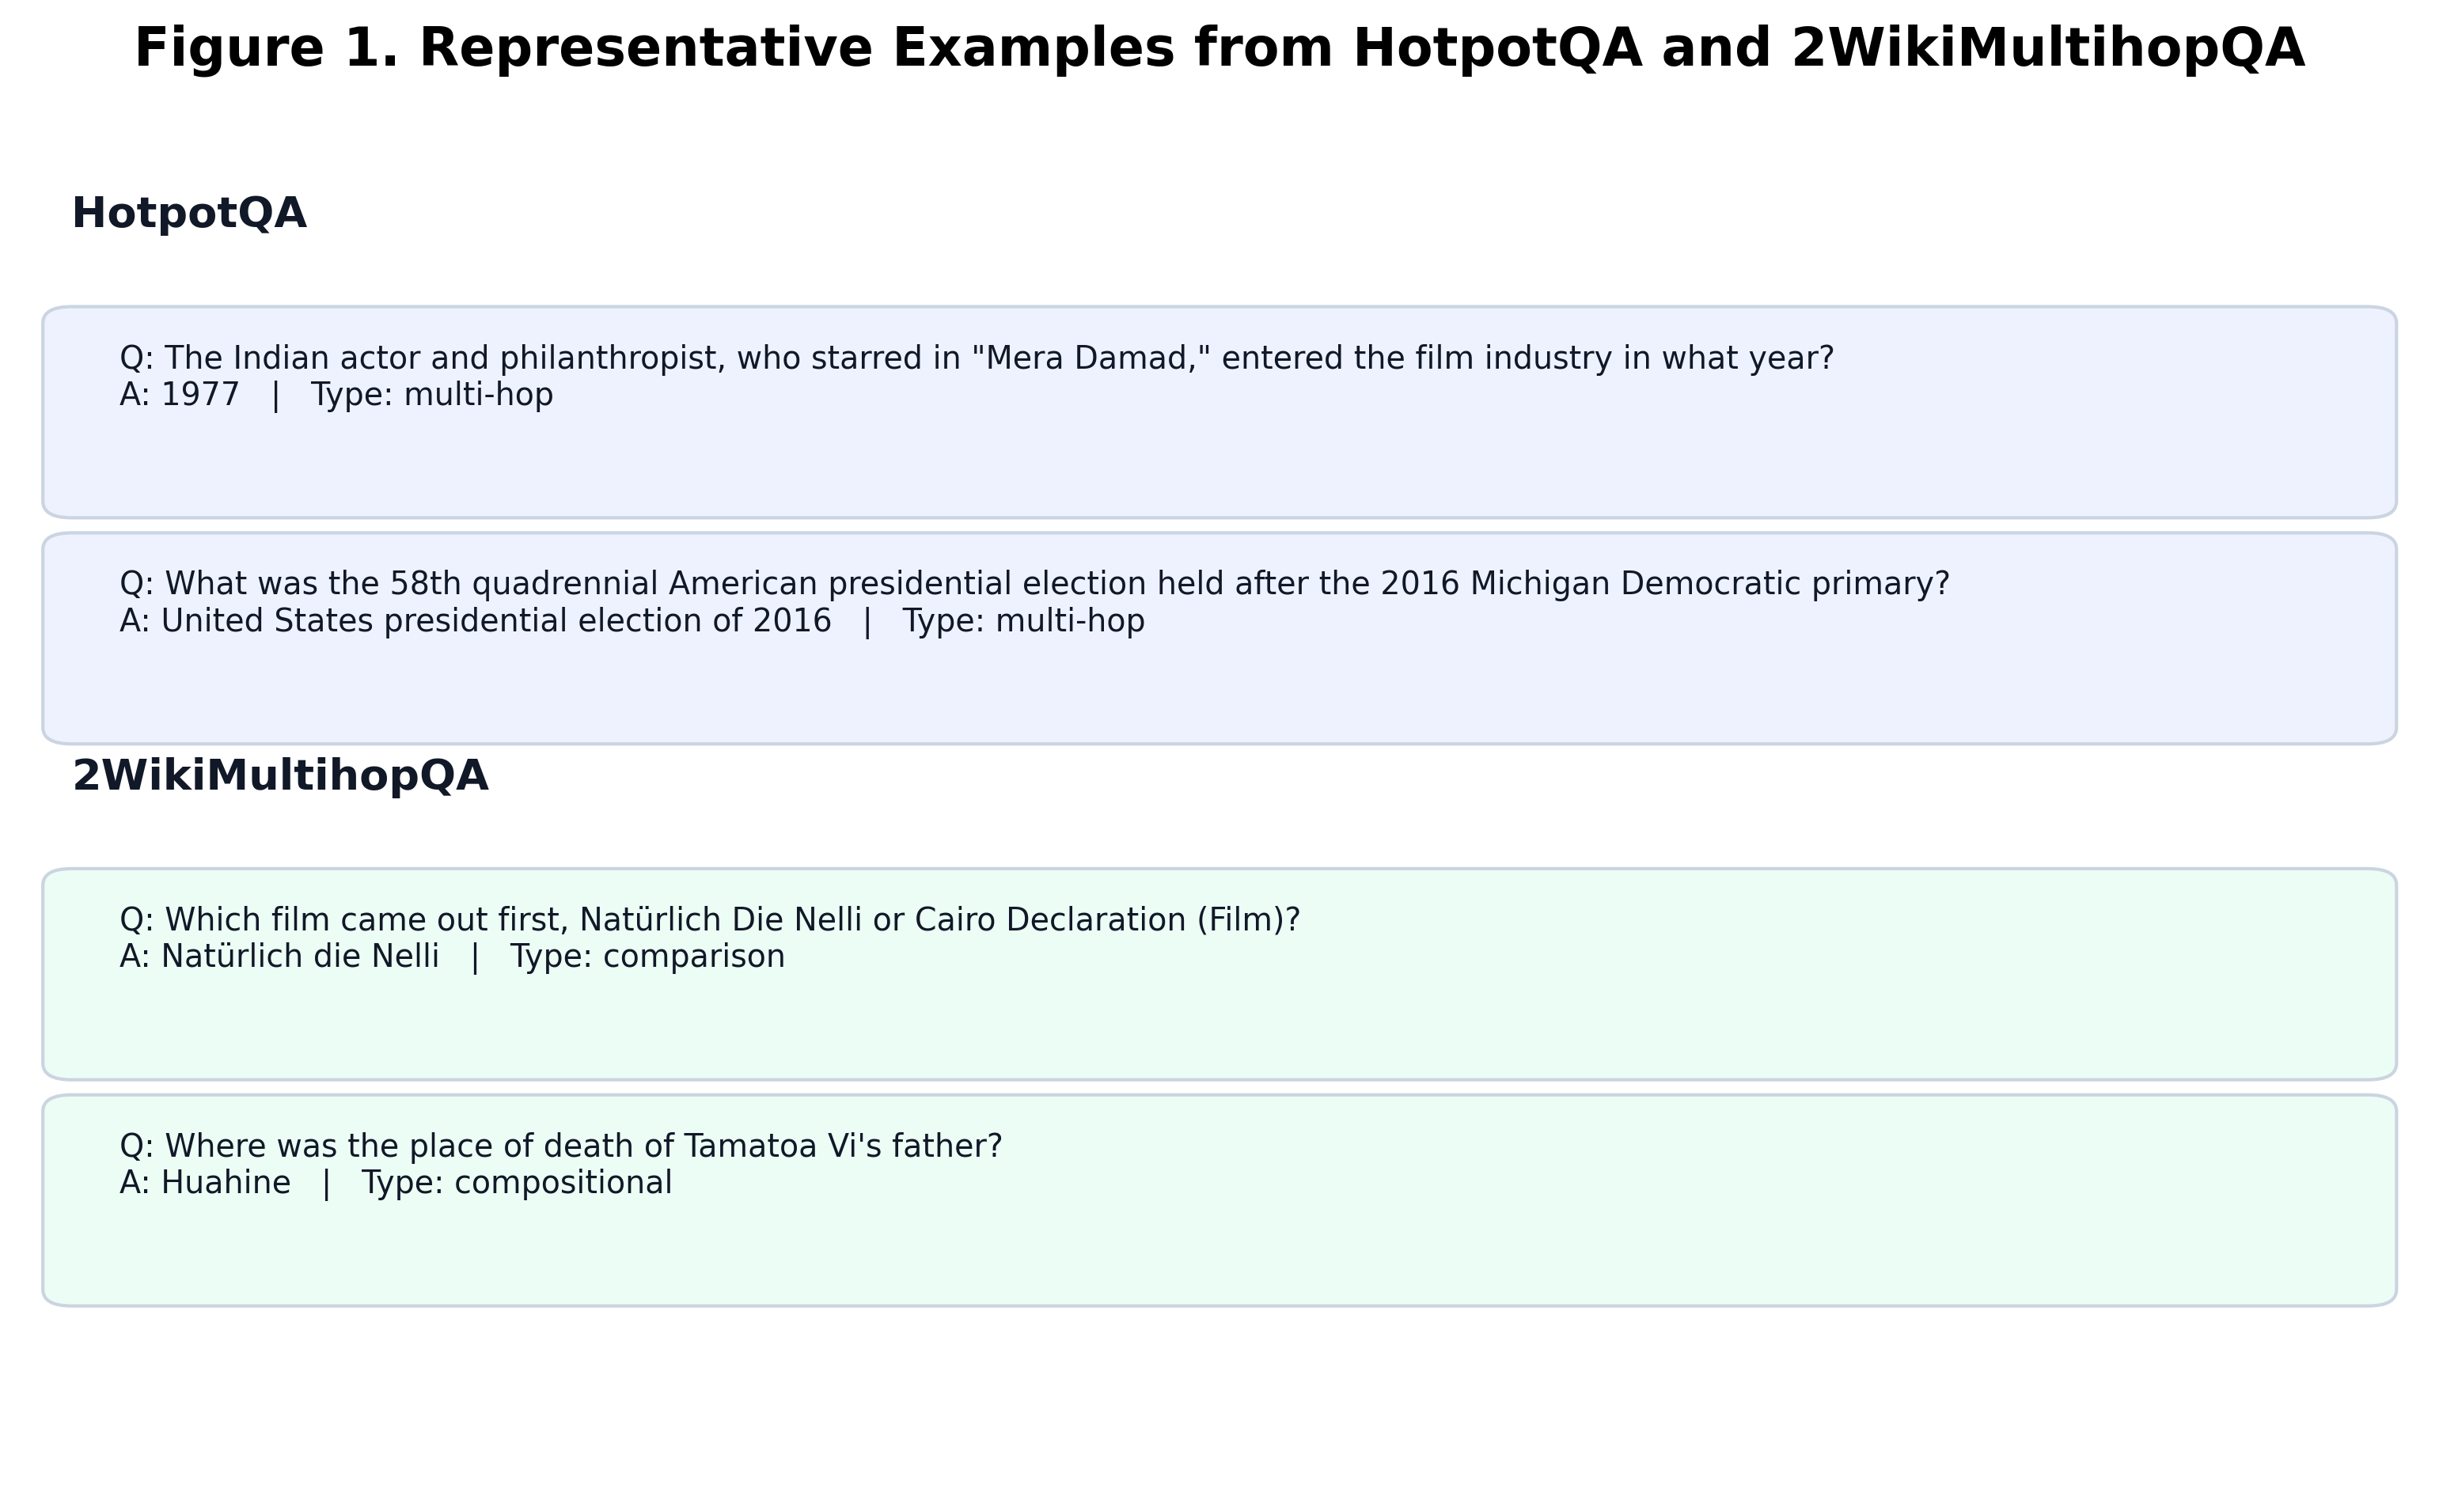
\includegraphics[width=0.88\linewidth]{figures/figure_1_dataset_examples.png}
\caption{Representative examples from HotpotQA and 2WikiMultihopQA datasets.}
\label{fig:dataset_examples}
\end{figure}
\vnote{Thêm hình minh họa 2--3 câu hỏi từ mỗi dataset, kèm evidence documents nếu muốn báo cáo trực quan hơn.}

\subsection{System Overview}

MAP-RAG-Gym consists of five connected components that should be shown explicitly in the system diagram: an input and budget interface, a macro workflow router, a workflow execution library, a micro process-critic layer, and an evaluation plus promotion-gate layer. The input side receives a natural-language multi-hop question together with a budget mode $b \in \{\text{low},\text{medium},\text{high}\}$. The budget mode is not only a display label; it changes the routing objective by changing the trade-off between answer quality and execution cost. The macro router therefore predicts a workflow rather than a single retrieval action. This design follows the principle of MAO-ARAG, but constrains the action space to a finite workflow library instead of allowing a planner model to freely generate arbitrary workflow strings. This choice improves reproducibility, makes offline evaluation possible, and reduces the risk of invalid or non-executable workflow formats.

The macro router uses several families of signals. First, it extracts lightweight question features such as WH-word type, token length, comparative indicators, conjunction indicators, ambiguity, temporal cues, negation, superlatives, multi-entity cues, entity density, and an estimated hop count. Second, it can incorporate a rule-based routing prior and a learned router prior. Third, when a probe retriever is attached, it uses retrieval-side signals such as top document scores, top-score gaps, document overlap, title overlap, and the number of retrieved documents. These features are converted into tabular and text features using TF--IDF, one-hot categorical encodings, and numeric features, and the bandit model predicts the expected utility for each candidate workflow. The selected workflow is the one with the highest predicted utility under the current budget and allowed workflow set.

The workflow execution layer implements six workflows. W1 performs direct answer generation and is therefore the cheapest workflow. W2 rewrites the query before retrieval and answer generation. W3 retrieves documents, selects evidence, and generates the answer. W4 and W5 represent parallel and serial decomposition patterns, respectively, although the reported final metrics focus mainly on W1, W2, W3, and W6. W6 uses a draft--reflect--retrieve--generate pattern and is inspired by the reflection mechanism emphasized in RAG-Gym. In the architecture figure, these workflows should be drawn as branches leaving the macro router and entering a shared execution engine. The shared execution engine calls local LLMs through Ollama, local retrievers such as BM25/TF--IDF/hybrid retrieval, and the dataset corpus. Each workflow returns a final answer, intermediate traces, and execution cost metadata including tokens, retrieval calls, and latency.

The micro critic layer sits inside the workflow execution layer rather than replacing the macro router. It is used at module level. For the QR module, the critic scores candidate rewritten queries and selects the candidate expected to improve retrieval. For the RA/DS path, the critic can rerank retrieved documents when a module-specific critic is available. For the AG module, the critic scores answer candidates and selects the candidate with stronger expected grounding and answer quality. Thus, the macro router chooses the coarse workflow, while the micro critic improves or diagnoses local decisions inside a chosen workflow. Finally, the evaluator receives the final answer, gold answer, process trace, and cost statistics. It computes EM, F1 proxy, process score, utility, regret, best-rate, and readiness gates. The promotion-gate block decides whether a learned router or critic setting is safe enough to be used in the final policy bundle.

\begin{table}[H]
\centering
\caption{Workflow library in MAP-RAG-Gym.}
\label{tab:workflow_library}
\begin{tabular}{lp{0.34\linewidth}p{0.43\linewidth}}
\toprule
\textbf{Workflow} & \textbf{Steps} & \textbf{Intended behavior} \\
\midrule
W1 & AG & Direct answer generation; lowest token and retrieval cost. \\
W2 & QR $\rightarrow$ RA $\rightarrow$ AG & Rewrite the question into a searchable form before retrieval and generation. \\
W3 & RA $\rightarrow$ DS $\rightarrow$ AG & Retrieve candidate documents, select useful evidence, and generate the answer. \\
W4 & QDP $\rightarrow$ RA $\rightarrow$ AS & Decompose independent sub-questions in parallel and synthesize the answer. \\
W5 & QDS $\rightarrow$ QR $\rightarrow$ RA $\rightarrow$ AS & Decompose dependent sub-questions sequentially and summarize sub-answers. \\
W6 & DRAFT $\rightarrow$ REFLECT $\rightarrow$ RA $\rightarrow$ AG & Draft an answer, identify missing evidence, retrieve, and regenerate. \\
\bottomrule
\end{tabular}
\end{table}

\begin{figure}[H]
\centering
% \includegraphics[width=0.92\linewidth]{figures/map_rag_gym_architecture.png}
\caption{Proposed MAP-RAG-Gym architecture with macro workflow routing, workflow library W1--W6, micro critics, evaluator, and promotion gates.}
\label{fig:model_architecture}
\end{figure}
\vnote{Khi vẽ Figure 2, nên bố cục từ trái sang phải. Khối 1 là Input Question + Budget Mode. Khối 2 là Feature Builder gồm question features, rule-router prior, learned-router prior, và optional probe-retrieval features. Khối 3 là Macro Bandit Router, xuất ra workflow W1--W6. Khối 4 là Workflow Execution Engine gồm các nhánh W1: AG; W2: QR--RA--AG; W3: RA--DS--AG; W4: QDP--RA--AS; W5: QDS--QR--RA--AS; W6: DRAFT--REFLECT--RA--AG. Khối 5 là Shared Resources gồm local Ollama LLMs, BM25/TF--IDF/Hybrid retrievers, và corpus HotpotQA/2WikiMultihopQA. Khối 6 là Micro Critics đặt bên trong các module QR, RA/DS, AG để rerank query/document/answer candidates. Khối 7 là Evaluator tính EM, F1, process score, cost, utility, regret, best-rate. Khối 8 là Promotion Gate/Policy Bundle quyết định cấu hình nào được triển khai. Nên dùng mũi tên feedback từ Evaluator về Router/Critic Training để thể hiện offline training loop.}

\subsection{Macro Budget-Aware Routing}

The macro router receives a question and a budget mode. The budget mode controls how aggressively the system should trade cost for answer quality. In low-budget mode, the system should prefer fewer tokens, fewer retrieval calls, and shorter latency. In medium-budget mode, it should allow moderate retrieval when the router expects utility gain. In high-budget mode, it can choose stronger workflows and accept higher cost if the expected answer quality improves. This mirrors the MAO-ARAG reward design, where the final reward combines answer quality with cost penalties \cite{chen2025maoarag}.

Let $q$ denote the input question, $b \in \{\text{low}, \text{medium}, \text{high}\}$ denote the budget mode, and $\mathcal{W}=\{W_1,\ldots,W_6\}$ denote the workflow set. The routing policy is written as
\begin{equation}
    W^{*} = \pi(q,b), \quad W^{*} \in \mathcal{W}.
\end{equation}
A workflow produces a predicted answer $\hat{a}$ and execution statistics such as tokens, retrieval calls, and latency. The utility used in the project is a scalar evaluation signal designed to reward answer quality while accounting for cost. Although the exact implementation is defined in the codebase, its role follows the general form
\begin{equation}
    U(q,W) = Q(\hat{a},a) - \lambda_b C(W),
\end{equation}
where $Q$ measures answer quality using EM, F1 proxy, and process-oriented signals, $C(W)$ summarizes execution cost, and $\lambda_b$ varies by budget mode.

\subsection{Micro Process Critic}

The micro layer follows the RAG-Gym argument that final-answer supervision alone is often too coarse for agentic RAG \cite{xiong2025raggym}. MAP-RAG-Gym therefore trains process critics for two modules: query rewriting (QR) and answer generation (AG). A process critic is a learned scoring function $r_\phi(s,a)$ that estimates the usefulness of an intermediate action $a$ under state $s$. For QR, the state contains the original question and context required to decide whether a rewritten query is useful. For AG, the state contains the question and retrieved evidence, while the action corresponds to an answer candidate.

The critic objective is conceptually related to preference modeling. Given a preferred action $a^+$ and a less preferred action $a^-$ for the same state $s$, a critic should assign a higher score to $a^+$. RAG-Gym describes this idea through a contrastive reward-modeling loss \cite{xiong2025raggym}. In MAP-RAG-Gym, critic performance is evaluated using regression and rank-correlation metrics, including MAE, RMSE, Pearson correlation, and Spearman correlation. A critic is considered safer for offline reward modeling when it ranks examples consistently with the target process signal.

\subsection{Experimental Setup}

The implementation is written in Python as a package under \texttt{src/map\_rag\_gym}. It includes executors, retrieval backends, routing logic, evaluation utilities, process critics, scripts for batch rollout, scripts for training and evaluation, and exported CSV metrics. All experiments use locally hosted open-source LLMs served through Ollama. Three models are used: Llama~3.2 (3B parameter), Gemma~3 (12B parameter), and Gemma~3 (4B parameter). No cloud API (e.g.~Gemini) is used in the reported experiments, although the codebase supports it. Each model is paired with each dataset, yielding five experimental configurations: HotpotQA$\times$Llama~3.2, HotpotQA$\times$Gemma~3, HotpotQA$\times$Gemma~3~(4B), 2WikiMultihopQA$\times$Gemma~3, and 2WikiMultihopQA$\times$Llama~3.2. This design lets the report compare not only budget-level trade-offs but also how different model capacities and dataset distributions interact with adaptive routing. The full pipeline (rollout, router training, critic training, evaluation, bandit tuning, RL gating, and metric export) is run independently for each configuration. Metrics are exported under \texttt{outputs/<config>/metrics/}.

\begin{table}[H]
\centering
\caption{Main implementation and experimental settings.}
\label{tab:training_settings}
\begin{tabular}{ll}
\toprule
\textbf{Setting} & \textbf{Value} \\
\midrule
Programming language & Python \\
Project package & \texttt{map\_rag\_gym} \\
Primary task & Multi-hop question answering \\
Datasets & HotpotQA, 2WikiMultihopQA \\
Dataset split (each) & 420 train / 90 validation / 90 test \\
Routing modes & low, medium, high \\
Workflow set & W1--W6 \\
Micro critics & QR critic and AG critic \\
LLM inference & Ollama (local only) \\
Models & Llama~3.2 (3B), Gemma~3 (12B), Gemma~3 (4B) \\
Experiment configs & 5 (dataset $\times$ model combinations) \\
Reported metric source & \texttt{outputs/<config>/metrics/*.csv} \\
\bottomrule
\end{tabular}
\end{table}

\subsection{Evaluation Metrics}

The report evaluates answer quality using exact match (EM), F1 proxy, and process score. EM captures whether the predicted answer exactly matches the gold answer after normalization. F1 proxy measures token-level overlap between prediction and reference answer. Process score measures internal step quality and is especially relevant for the critic layer. Because the project is budget-aware, answer metrics alone are insufficient; therefore, token count, retrieval calls, and latency are also reported.

For binary or token-overlap answer evaluation, the usual precision, recall, and F1 definitions are
\begin{equation}
    \text{Precision} = \frac{TP}{TP + FP}, \quad
    \text{Recall} = \frac{TP}{TP + FN},
\end{equation}
\begin{equation}
    F1 = 2 \times \frac{\text{Precision} \times \text{Recall}}{\text{Precision} + \text{Recall}}.
\end{equation}
For bandit routing, regret measures the loss relative to the oracle workflow selection, while best-rate measures how often the bandit selects the empirically best workflow. For critic evaluation, Spearman correlation is particularly important because the critic is used primarily to rank candidate actions.

\section{Results}

\subsection{Budget-Aware Macro Routing}

Table~\ref{tab:budget_summary} reports the main held-out results for the three budget modes using HotpotQA with Llama~3.2, which serves as the primary experimental configuration. The trend is consistent with the intended system design. Higher budget modes produce higher utility and better answer-quality proxies, but they also require more tokens and longer latency. Low-budget routing uses 104.46 tokens on average and obtains a utility of 0.2776. High-budget routing increases average token use to 176.53 and latency to 1151.62~ms, but also improves utility to 0.4375 and F1 proxy to 0.3220. This result supports the central claim that routing should not be evaluated only by answer quality; it should be interpreted as a quality--cost trade-off.

\begin{table}[H]
\centering
\caption{Budget-aware macro routing on HotpotQA with Llama~3.2 (primary configuration).}
\label{tab:budget_summary}
\resizebox{\linewidth}{!}{%
\begin{tabular}{l l c c c c c c c}
\toprule
\textbf{Budget} & \textbf{Method} & \textbf{Runs} & \textbf{Utility} & \textbf{EM} & \textbf{F1 proxy} & \textbf{Tokens} & \textbf{Retrieval calls} & \textbf{Latency (ms)} \\
\midrule
Low & gated\_bandit\_router & 90 & 0.2776 & 0.2222 & 0.2720 & 104.46 & 0.72 & 761.99 \\
Medium & bandit\_router & 90 & 0.3613 & 0.2444 & 0.3011 & 116.40 & 0.60 & 907.93 \\
High & bandit\_router & 90 & 0.4375 & 0.2778 & 0.3220 & 176.53 & 1.00 & 1151.62 \\
\bottomrule
\end{tabular}%
}
\end{table}

\subsection{Cross-Model and Cross-Dataset Comparison}

To evaluate how adaptive routing behaves across different LLMs and question distributions, the complete pipeline was run on five configurations. Table~\ref{tab:cross_model_dataset} summarizes the final selected policy performance per budget across all configurations. HotpotQA consistently yields higher utility than 2WikiMultihopQA, which is expected given that 2WikiMultihopQA contains more structurally complex reasoning patterns including bridge and comparison questions. Among models, Llama~3.2 on HotpotQA achieves the highest high-budget utility (0.4375), significantly outperforming Gemma~3 variants on the same dataset. Interestingly, Gemma~3 (4B) on HotpotQA obtains a higher high-budget utility (0.2578) than Gemma~3 (12B) on HotpotQA (0.2733), though both are well below Llama~3.2. On 2WikiMultihopQA, Llama~3.2 achieves high-budget utility of 0.1816 and Gemma~3 reaches 0.1778, confirming the dataset's greater difficulty. A notable observation is that the gap between low-budget and high-budget utility varies: on HotpotQA with Llama~3.2, the gap is +0.1599, whereas on 2WikiMultihopQA with Llama~3.2, the gap is only +0.0276, suggesting that budget-aware routing benefits some dataset--model combinations more than others.

\begin{table}[H]
\centering
\caption{Cross-model and cross-dataset comparison: final selected policy per budget (held-out test, 90 questions).}
\label{tab:cross_model_dataset}
\resizebox{\linewidth}{!}{%
\begin{tabular}{l l c c c c c c c c c}
\toprule
\textbf{Dataset} & \textbf{Model} & \multicolumn{3}{c}{\textbf{Low budget}} & \multicolumn{3}{c}{\textbf{Medium budget}} & \multicolumn{3}{c}{\textbf{High budget}} \\
\cmidrule(lr){3-5} \cmidrule(lr){6-8} \cmidrule(lr){9-11}
 & & \textbf{Utility} & \textbf{EM} & \textbf{F1} & \textbf{Utility} & \textbf{EM} & \textbf{F1} & \textbf{Utility} & \textbf{EM} & \textbf{F1} \\
\midrule
HotpotQA & Llama~3.2 (3B) & \textbf{0.2776} & 0.2222 & 0.2720 & \textbf{0.3613} & 0.2444 & 0.3011 & \textbf{0.4375} & 0.2778 & 0.3220 \\
HotpotQA & Gemma~3 (12B) & 0.1798 & 0.1000 & 0.1877 & 0.2346 & 0.1000 & 0.1824 & 0.2733 & 0.1000 & 0.1824 \\
HotpotQA & Gemma~3 (4B) & 0.1511 & 0.0889 & 0.1715 & 0.2176 & 0.0889 & 0.1715 & 0.2578 & 0.0889 & 0.1715 \\
2WikiMultihopQA & Gemma~3 (12B) & 0.1107 & 0.0778 & 0.1068 & 0.1478 & 0.0667 & 0.1201 & 0.1778 & 0.0667 & 0.1181 \\
2WikiMultihopQA & Llama~3.2 (3B) & 0.1540 & 0.1222 & 0.1448 & 0.1704 & 0.1222 & 0.1448 & 0.1816 & 0.1222 & 0.1448 \\
\bottomrule
\end{tabular}%
}
\end{table}

\begin{figure}[H]
\centering
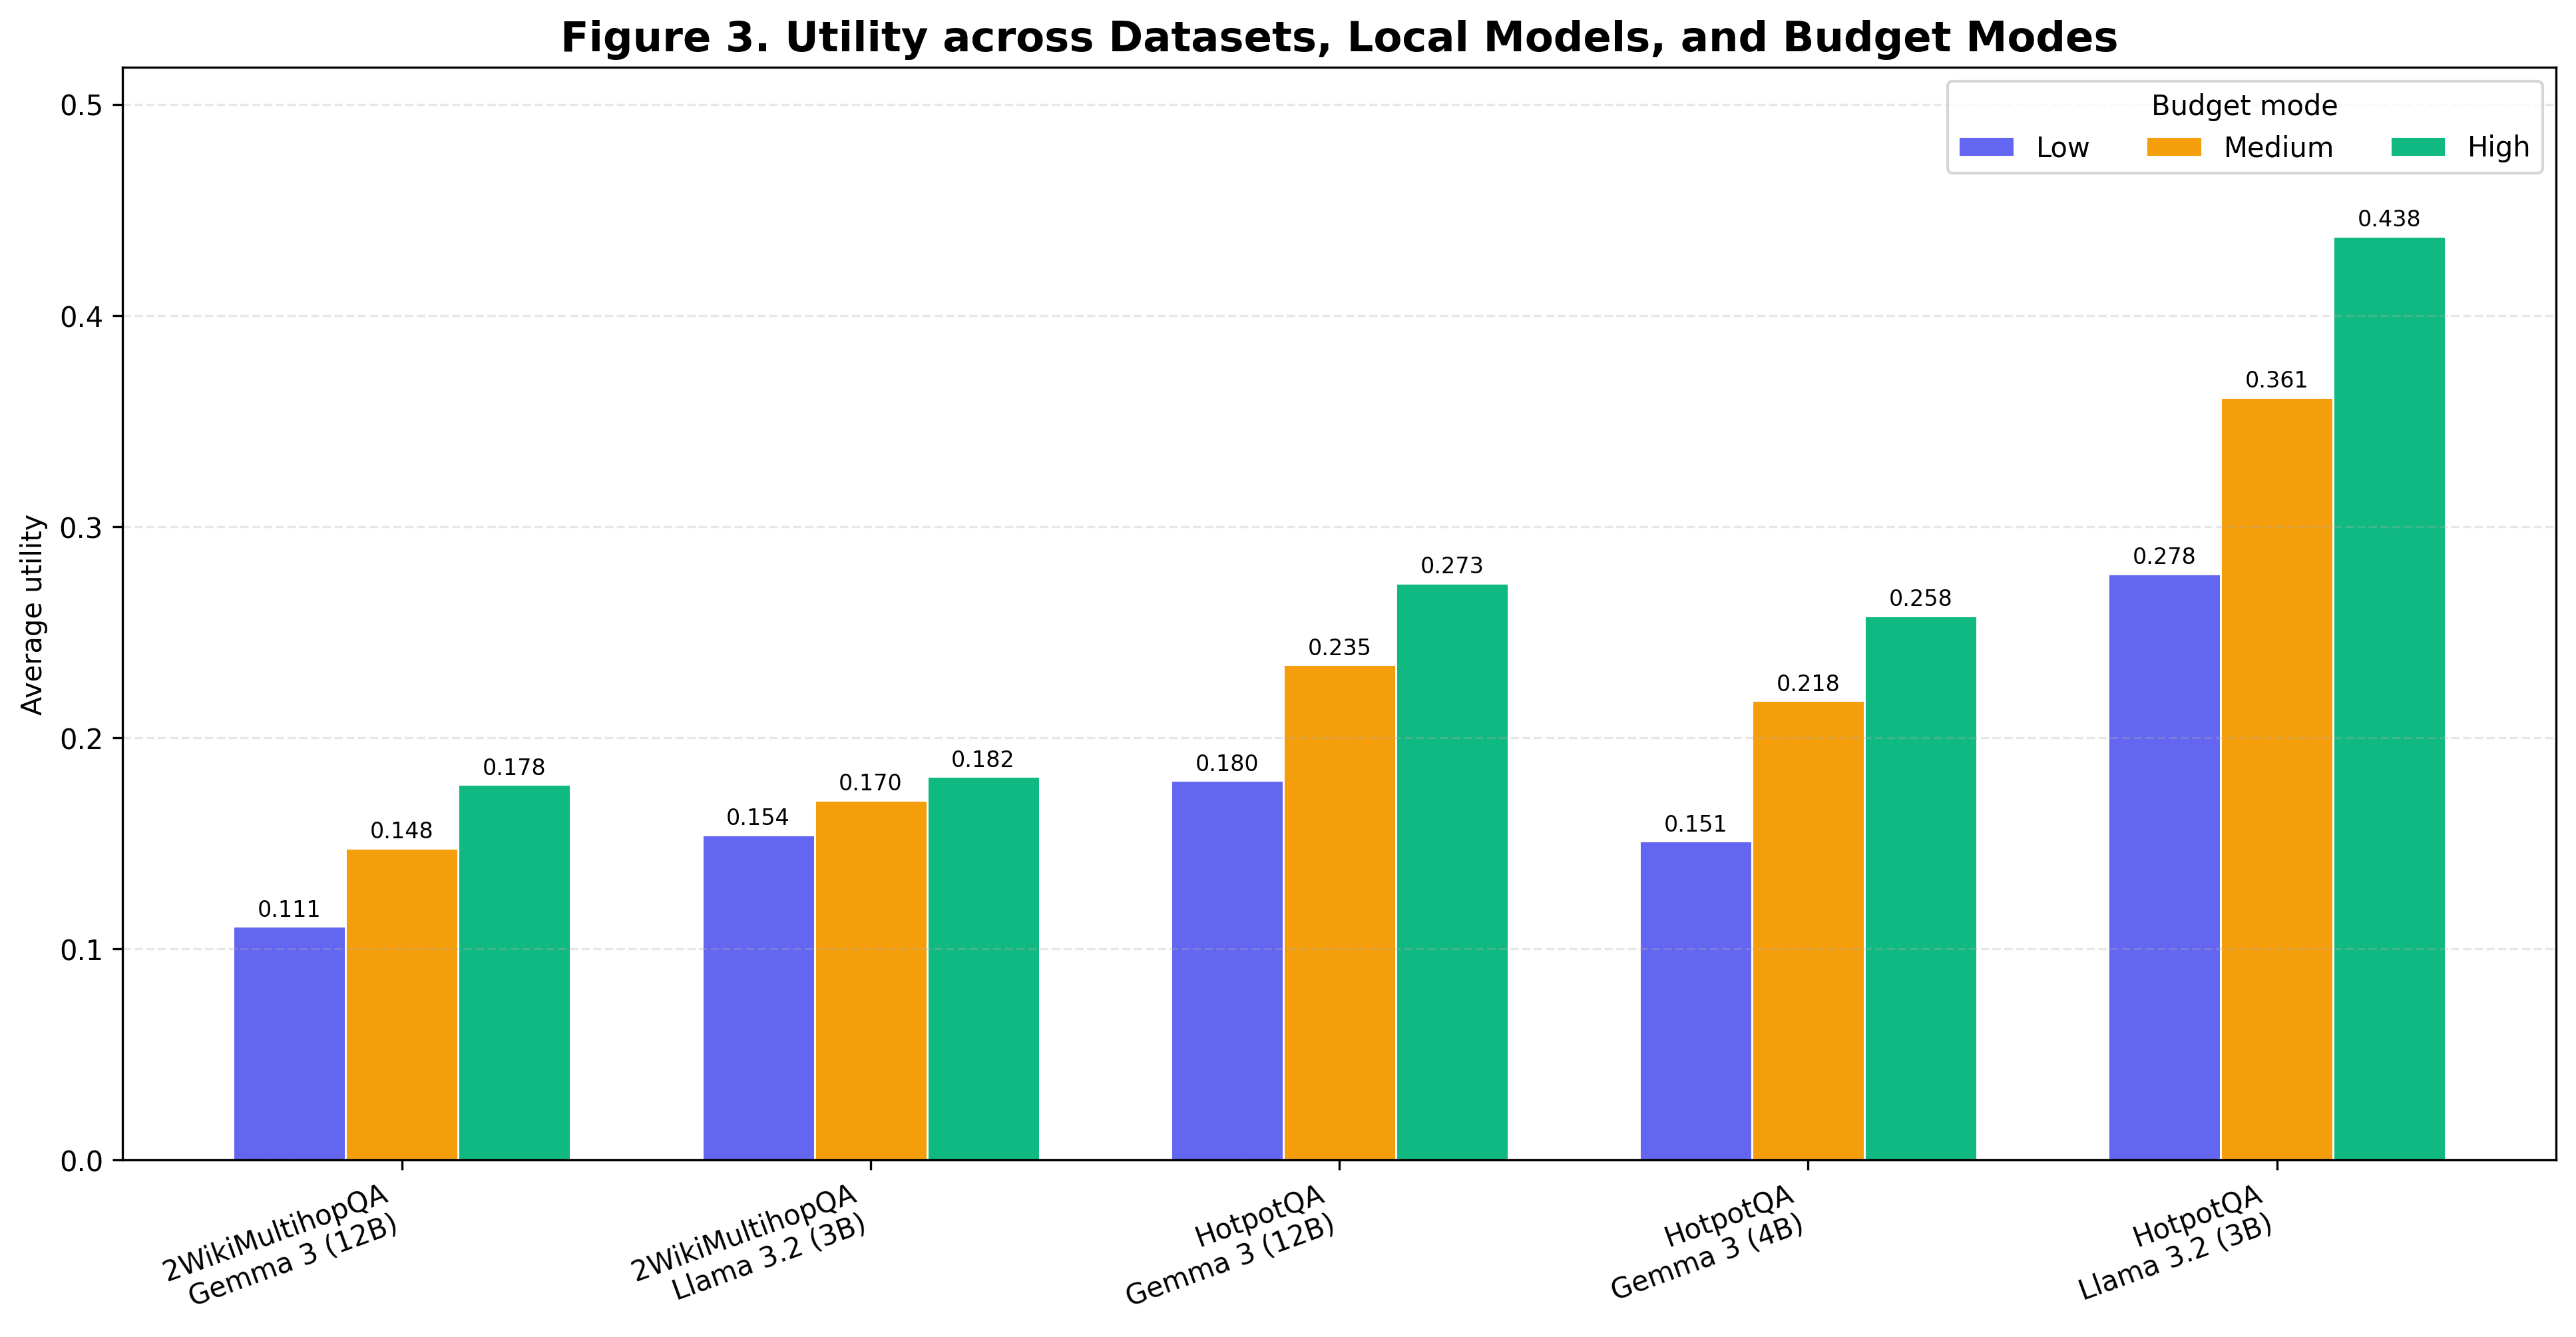
\includegraphics[width=0.92\linewidth]{figures/figure_3_budget_utility.png}
\caption{Suggested grouped bar chart comparing utility across all five configurations and three budget modes.}
\label{fig:budget_chart}
\end{figure}
\vnote{Tạo biểu đồ cột nhóm: trục x là 5 cấu hình (dataset × model); nhóm 3 cột low/medium/high cho mỗi cấu hình. Có thể dùng matplotlib hoặc Streamlit app để tạo.}

\subsection{Workflow Selection Behavior}

The workflow distribution varies meaningfully across configurations. On HotpotQA with Llama~3.2, the low-budget router allocates W1 to 25 questions and W3 to 65. The high-budget policy eliminates W1 entirely and focuses on W2 (37) and W3 (53). On the same dataset with Gemma~3 (12B), medium-budget routing becomes more diverse, assigning 23 questions to W6 (reflective retrieval), indicating that the larger model benefits from reflection workflows. On 2WikiMultihopQA, the router also uses multiple workflows, but the overall utility is lower, reflecting the dataset's greater difficulty rather than a routing failure.

This adaptive distribution is the core project contribution: instead of running one fixed pipeline, the system adjusts behavior by budget mode, model capacity, and question distribution. The retrieval and evidence-selection workflows become more attractive when the budget allows higher cost.

\subsection{Fixed Workflow and Critic Deployment Comparison}

Table~\ref{tab:fixed_workflow_comparison} compares representative fixed workflows and learned routing variants. W3 is the strongest fixed workflow among the shown non-critic baselines, with utility 0.4187 and F1 proxy 0.3100. W2 is more expensive, consuming 243.12 tokens on average, while W1 is cheap but substantially weaker. The learned router obtains utility 0.4050 with a mix of W2, W3, W6, and W1, but its critic-augmented version decreases utility and more than doubles token usage. This result is an important negative finding: critic guidance can be useful only when applied selectively and safely; always enabling critic-based reranking may create unnecessary cost without improving answer quality.

\begin{table}[H]
\centering
\caption{Selected fixed workflow and critic-deployment results.}
\label{tab:fixed_workflow_comparison}
\resizebox{\linewidth}{!}{%
\begin{tabular}{l c c c c c c c}
\toprule
\textbf{Method} & \textbf{Critic} & \textbf{Utility} & \textbf{EM} & \textbf{F1 proxy} & \textbf{Tokens} & \textbf{Retrieval calls} & \textbf{Latency (ms)} \\
\midrule
fixed\_W1 & no & 0.2091 & 0.1111 & 0.1707 & 41.12 & 0.00 & 1041.01 \\
fixed\_W2 & no & 0.3940 & 0.2111 & 0.3013 & 243.12 & 1.00 & 2842.26 \\
fixed\_W3 & no & 0.4187 & 0.2000 & 0.3100 & 121.84 & 1.00 & 1150.26 \\
fixed\_W3\_critic & yes & 0.4239 & 0.2111 & 0.3137 & 121.84 & 1.00 & 1082.15 \\
fixed\_W6 & no & 0.3697 & 0.2000 & 0.2889 & 300.46 & 1.00 & 4423.18 \\
learned\_router & no & 0.4050 & 0.2111 & 0.3065 & 218.42 & 0.99 & 2759.71 \\
learned\_router\_critic & yes & 0.3915 & 0.2111 & 0.3065 & 522.04 & 0.99 & 5221.17 \\
\bottomrule
\end{tabular}%
}
\end{table}

\subsection{Micro Critic Quality}

Table~\ref{tab:critic_quality} reports critic quality across configurations. In most configurations that share the same HotpotQA-based training data, the QR critic reaches Pearson 0.7050 and Spearman 0.6745. The best critic performance is observed on HotpotQA with Gemma~3 (4B), where QR achieves Spearman 0.7701 and AG reaches 0.4127---the only configuration where the AG critic is also marked ready as an offline reward model. This suggests that model capacity and data characteristics interact meaningfully with critic training: a smaller model with more consistent behavior may produce more predictable process signals.

\begin{table}[H]
\centering
\caption{Micro critic quality across experimental configurations.}
\label{tab:critic_quality}
\resizebox{\linewidth}{!}{%
\begin{tabular}{l l l c c c c c c}
\toprule
\textbf{Dataset} & \textbf{Model} & \textbf{Module} & \textbf{Train ex.} & \textbf{Eval ex.} & \textbf{MAE} & \textbf{RMSE} & \textbf{Pearson} & \textbf{Spearman} \\
\midrule
\multirow{2}{*}{HotpotQA} & \multirow{2}{*}{Llama~3.2} & QR & 1071 & 189 & 0.0955 & 0.1202 & 0.7050 & 0.6745 \\
 & & AG & 4283 & 756 & 0.2203 & 0.2950 & 0.2987 & 0.2112 \\
\midrule
\multirow{2}{*}{HotpotQA} & \multirow{2}{*}{Gemma~3 (12B)} & QR & 1071 & 189 & 0.0955 & 0.1202 & 0.7050 & 0.6745 \\
 & & AG & 4283 & 756 & 0.2203 & 0.2950 & 0.2987 & 0.2112 \\
\midrule
\multirow{2}{*}{HotpotQA} & \multirow{2}{*}{Gemma~3 (4B)} & QR & 1071 & 189 & \textbf{0.0839} & \textbf{0.1060} & \textbf{0.7525} & \textbf{0.7701} \\
 & & AG & 4284 & 756 & \textbf{0.1489} & \textbf{0.2335} & \textbf{0.4152} & \textbf{0.4127} \\
\midrule
\multirow{2}{*}{2WikiMultihopQA} & \multirow{2}{*}{Gemma~3 (12B)} & QR & 1071 & 189 & 0.0955 & 0.1202 & 0.7050 & 0.6745 \\
 & & AG & 4283 & 756 & 0.2203 & 0.2950 & 0.2987 & 0.2112 \\
\midrule
\multirow{2}{*}{2WikiMultihopQA} & \multirow{2}{*}{Llama~3.2} & QR & 1071 & 189 & 0.0955 & 0.1202 & 0.7050 & 0.6745 \\
 & & AG & 4283 & 756 & 0.2203 & 0.2950 & 0.2987 & 0.2112 \\
\bottomrule
\end{tabular}%
}
\end{table}

The critic comparison provides one of the clearest contributions of the project. MAP-RAG-Gym does not simply report whether RAG answers are correct; it exposes whether internal process modules can be evaluated with learned signals. The QR critic result suggests that process-level evaluation is feasible for at least some RAG components. The Gemma~3 (4B) result further shows that even the AG critic can become usable given the right model--data combination, while the weaker AG performance elsewhere defines a concrete limitation and future improvement target.

\subsection{High-Budget Bandit and System Gates}

The high-budget routing problem is particularly important because the system must decide between stronger retrieval-based workflows. In this setting, the main candidates are W2 and W3. W2 first rewrites the query and then retrieves evidence, while W3 retrieves first, selects documents, and then generates the answer. Both workflows are more expensive than direct generation, but they can produce better answers when retrieval is useful. The high-budget bandit is therefore trained as an offline contextual bandit: for each training question, previous workflow rollouts provide the observed utility of each candidate workflow; the router learns to predict this utility from question features, routing priors, and optional probe-retrieval features, and then selects the workflow with the highest predicted reward.

The cross-validation experiment in Figure~\ref{fig:bandit_cv_chart} is designed to reduce overfitting risk when selecting this high-budget router. Instead of choosing a configuration from a single train--holdout split, the script performs $K$-fold cross-validation over questions. In each fold, the model is trained on $K-1$ folds and evaluated on the held-out fold. The reported regret and best-rate are then averaged across folds, and their standard deviations measure stability. The search compares Ridge bandit models, Gradient Boosting Tree (GBT) bandit models, and ensembles that blend Ridge and GBT predicted utilities. Ridge provides a regularized linear baseline over sparse TF--IDF, categorical, and numeric features, while GBT captures nonlinear interactions such as when a comparative, multi-entity question benefits from one retrieval workflow more than another. The ensemble score is computed by blending the two predicted utility scores, using a blend parameter $\alpha$.

Table~\ref{tab:bandit_system_gates} summarizes the exported system gates. The bandit gate reports average regret of 0.0352 and exact best-rate of 0.8047, satisfying the online threshold. Figure~\ref{fig:bandit_cv_chart} gives the model-selection view behind this gate. In the top cross-validation table, \texttt{cv\_avg\_regret} is the average utility lost relative to the oracle workflow that would have selected the best observed workflow for each question. Lower regret is better. \texttt{cv\_avg\_best\_rate} is the fraction of questions for which the bandit selected exactly the same workflow as the oracle. Higher best-rate is better. The standard-deviation columns indicate whether performance is stable across folds. The selected best configuration, \texttt{ens\_ra10.0\_n150\_d4\_lr005\_b0.4}, is an ensemble with Ridge regularization $\alpha=10.0$, a GBT component with 150 estimators, maximum depth 4, learning rate 0.05, and blend weight 0.4. It obtains the highest cross-validated best-rate of 0.8333 with low regret of 0.0193. This means that the router matches the oracle workflow on about 83.33\% of validation questions while losing only about 0.0193 utility on average when it does not choose the oracle. The result supports the contribution that a small, interpretable workflow library can be made adaptive through offline bandit selection without requiring online exploration during evaluation.

The critic gate is also marked as passing in the exported system overview, and the final deployment mode is \texttt{selective\_critic\_online}. These results do not mean that an online learning loop has already been fully executed in production; rather, they show that the project has cleared the predefined readiness checks for moving toward online full-system reinforcement learning.

\begin{table}[H]
\centering
\caption{System-level online readiness metrics from exported overview.}
\label{tab:bandit_system_gates}
\begin{tabular}{l l l}
\toprule
\textbf{Category} & \textbf{Metric} & \textbf{Value} \\
\midrule
RL Gate & online\_rl\_ready & True \\
RL Gate & deployment\_mode & selective\_critic\_online \\
RL Gate & recommended\_next\_stage & online\_full\_system\_rl\_with\_selective\_critic \\
Bandit Gate & avg\_regret & 0.0352 \\
Bandit Gate & exact\_best\_rate & 0.8047 \\
Bandit Gate & meets\_online\_threshold & True \\
Critic Gate & token\_multiplier & 1.0 \\
Critic Gate & utility\_gap & 0.0 \\
Critic Gate & meets\_online\_threshold & True \\
Promotion & promoted & True \\
\bottomrule
\end{tabular}
\end{table}

\begin{figure}[H]
\centering
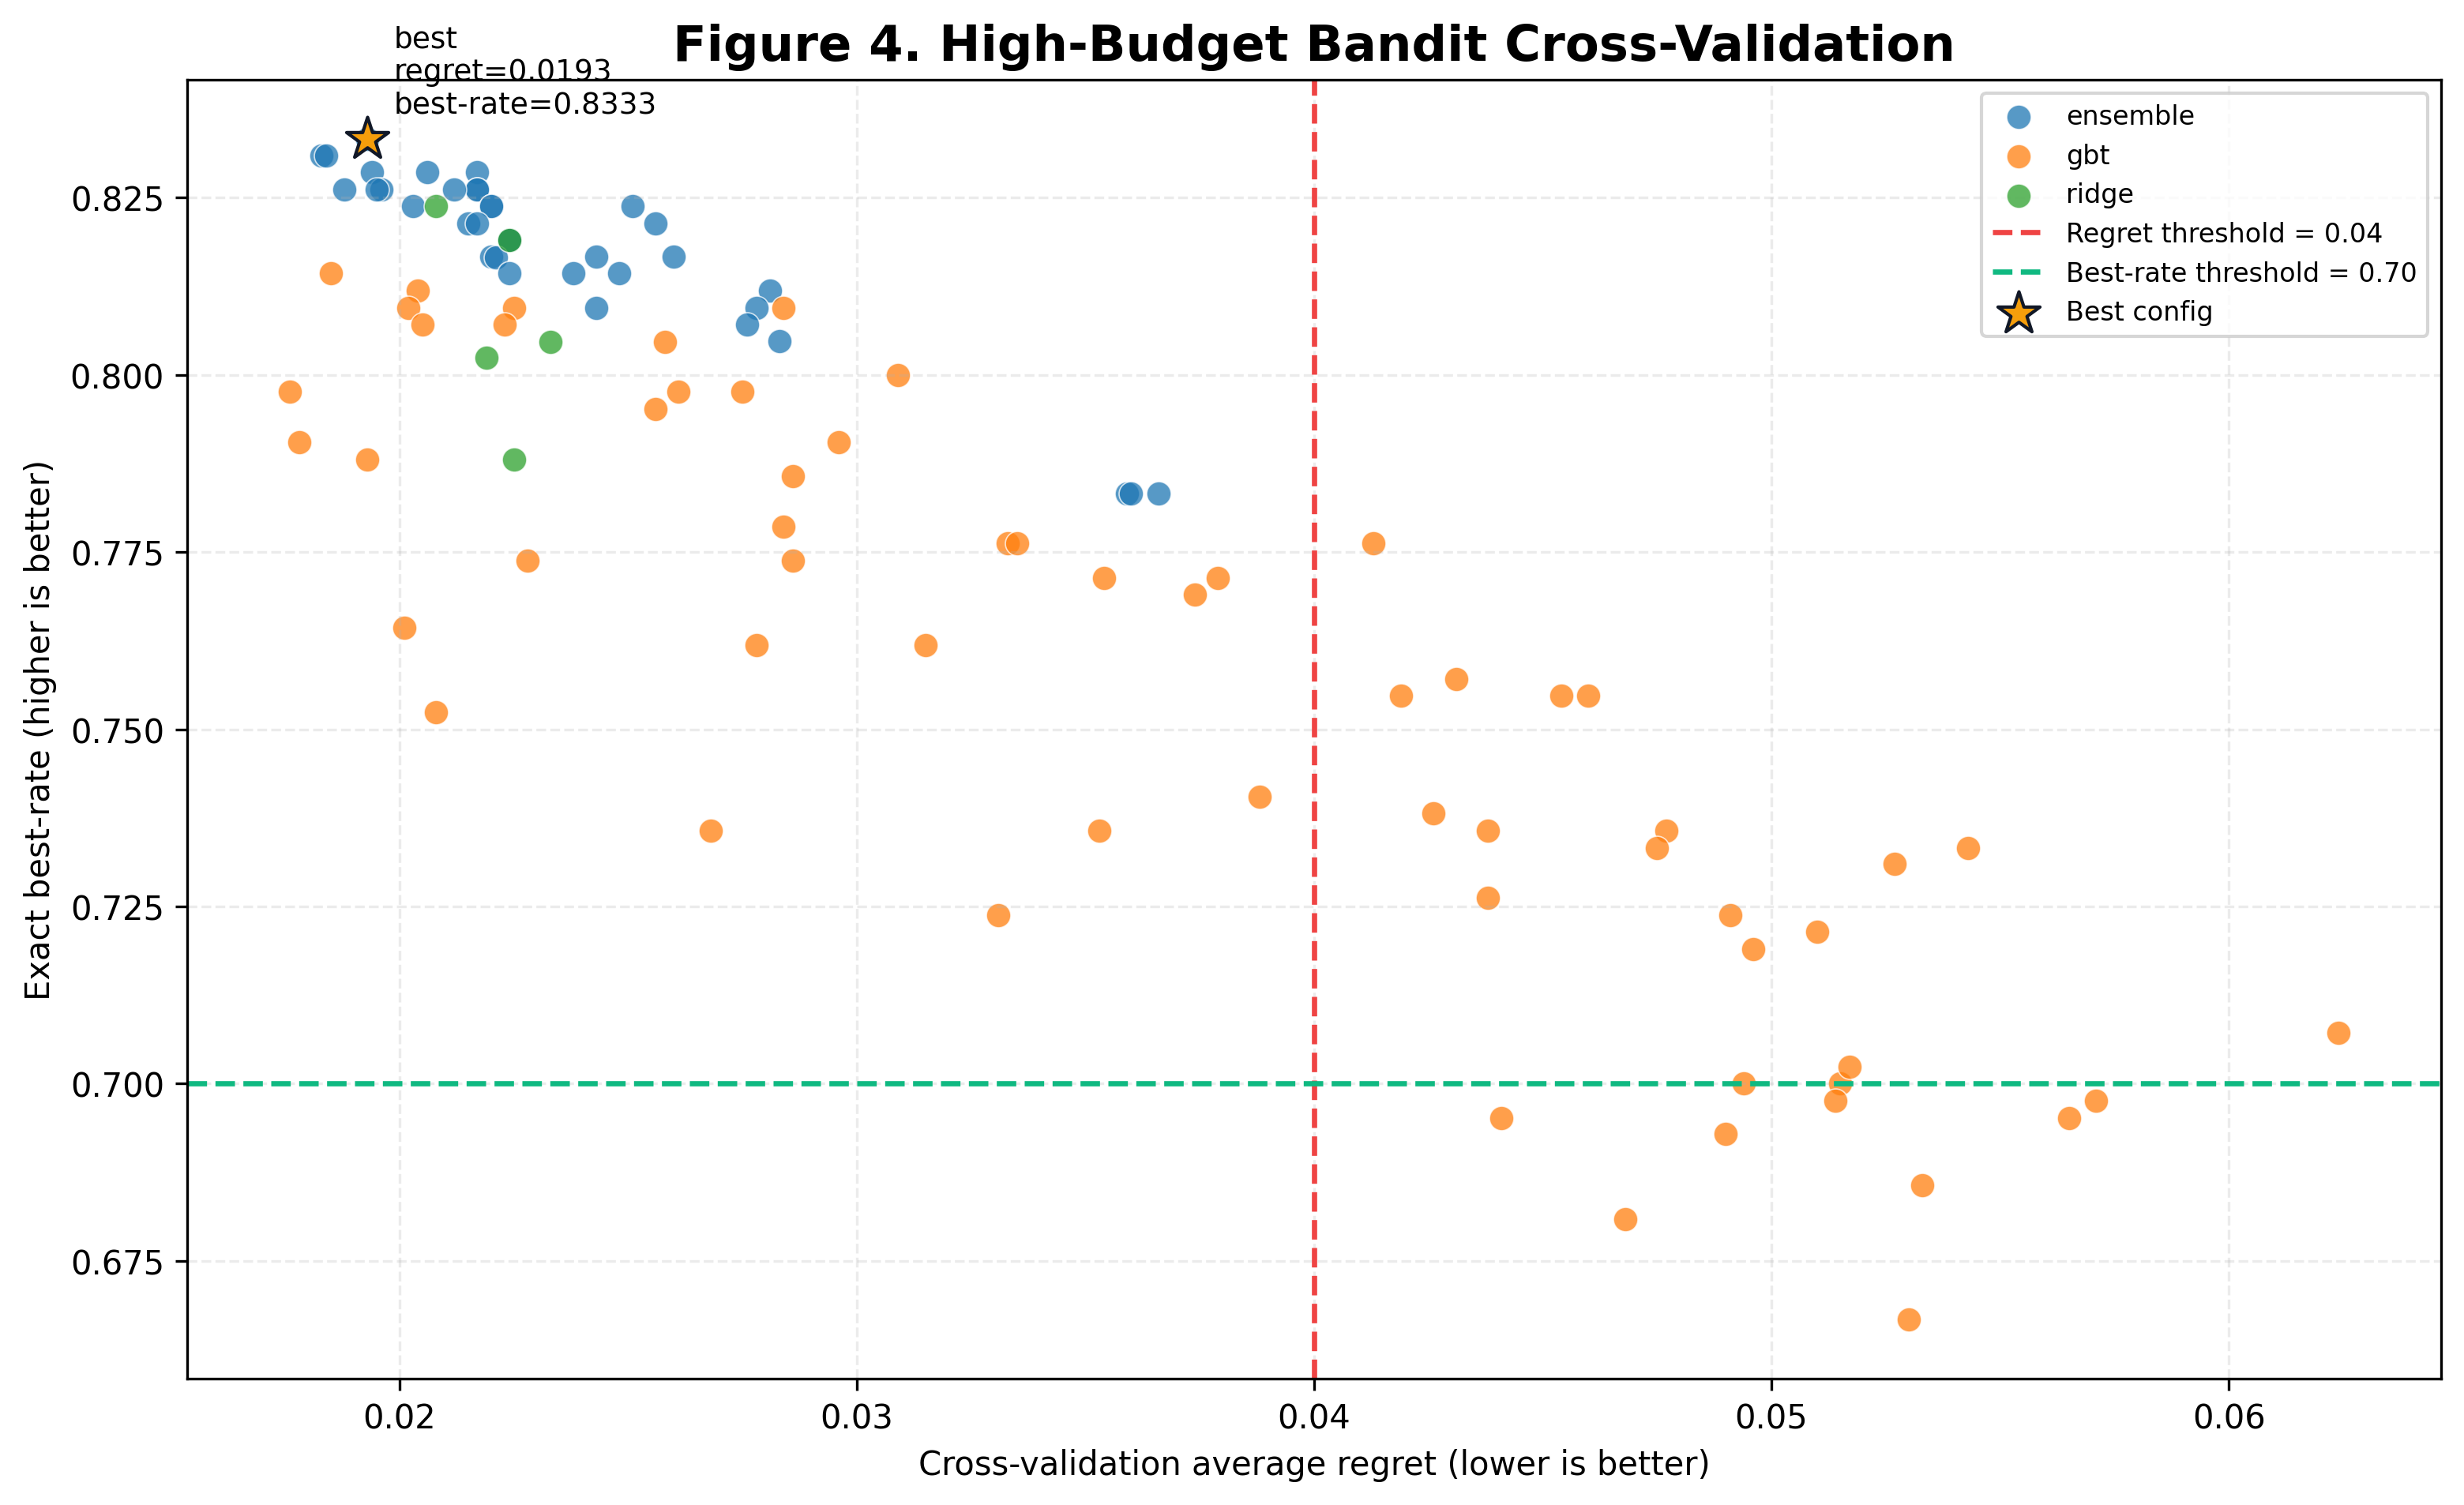
\includegraphics[width=0.88\linewidth]{figures/figure_4_bandit_cv.png}
\caption{High-budget bandit cross-validation over candidate router configurations. Each point represents one trained configuration. The x-axis reports cross-validated regret, where lower is better, and the y-axis reports exact best-rate, where higher is better. The highlighted best configuration is \texttt{ens\_ra10.0\_n150\_d4\_lr005\_b0.4}.}
\label{fig:bandit_cv_chart}
\end{figure}
\vnote{Figure 4 cần nhấn mạnh rằng đây là mô hình chọn cấu hình router bằng 5-fold cross-validation trên các câu hỏi training rollout. Mỗi cấu hình được train trên 4 folds và test trên 1 fold, lặp qua toàn bộ folds. Best config không chọn theo regret thấp nhất đơn lẻ mà theo mục tiêu cân bằng: best-rate cao, regret thấp, và variance nhỏ. Trong bảng top 10, cấu hình \texttt{ens\_ra10.0\_n150\_d4\_lr005\_b0.4} là tốt nhất vì đạt \texttt{cv\_avg\_best\_rate}=0.8333, \texttt{cv\_avg\_regret}=0.0193, \texttt{cv\_std\_regret}=0.0103, và \texttt{cv\_std\_best\_rate}=0.0404. Nên diễn giải: best-rate cho biết tỉ lệ chọn đúng workflow oracle, regret cho biết mất mát utility trung bình so với oracle, std cho biết độ ổn định giữa folds.}

\subsection{Selective Critic Verification}

The selective critic experiment provides a safety-oriented view of process critic deployment. Table~\ref{tab:selective_critic} shows that always using the critic leads to higher token usage and lower utility relative to the base method. With threshold 0.0, the critic is used on all 90 examples, token multiplier reaches 2.3901, and utility drops by 0.0135 relative to base. At threshold 1.0, the critic is never used, token multiplier is 1.0, and utility gap is 0.0. The result supports a conservative conclusion: in the current project state, the critic is more reliable as an offline reward and analysis tool than as an always-on online reranker.

\begin{table}[H]
\centering
\caption{Selective critic verification on 90 held-out examples.}
\label{tab:selective_critic}
\resizebox{\linewidth}{!}{%
\begin{tabular}{c c c c c c c}
\toprule
\textbf{Gate} & \textbf{Critic used} & \textbf{Critic skipped} & \textbf{Usage rate} & \textbf{Avg utility} & \textbf{Token multiplier} & \textbf{Meets both gates} \\
\midrule
0.00 & 90 & 0 & 1.0000 & 0.3915 & 2.3901 & no \\
0.50 & 74 & 16 & 0.8222 & 0.3946 & 2.1430 & no \\
0.70 & 89 & 1 & 0.9889 & 0.3917 & 2.3746 & no \\
1.00 & 0 & 90 & 0.0000 & 0.4050 & 1.0000 & yes \\
\bottomrule
\end{tabular}%
}
\end{table}

This table also clarifies why process critics should be guarded by deployment gates. RAG-Gym demonstrates that critic-guided action selection can improve agentic RAG when the critic is strong and inference sampling is appropriately designed \cite{xiong2025raggym}. MAP-RAG-Gym, however, shows that a smaller project implementation must verify critic behavior empirically before using it online. The contribution is therefore both positive and diagnostic: QR critic quality is promising, but indiscriminate critic deployment can be costly.

\subsection{Qualitative Results and Error Analysis}

The quantitative results suggest that MAP-RAG-Gym benefits from adaptive routing, but the system still has several error sources. Direct answering can fail when the model lacks the relevant fact. Query rewriting can fail when it removes a necessary entity or relation. Retrieval can return distracting documents, which makes document selection and answer generation harder. Reflective workflows can improve missing-evidence detection, but they also increase token usage and latency. These behaviors are consistent with observations in prior agentic RAG research, where multi-step retrieval improves complex reasoning but introduces additional opportunities for suboptimal intermediate actions \cite{yao2023react,xiong2025raggym}.

\begin{figure}[H]
\centering
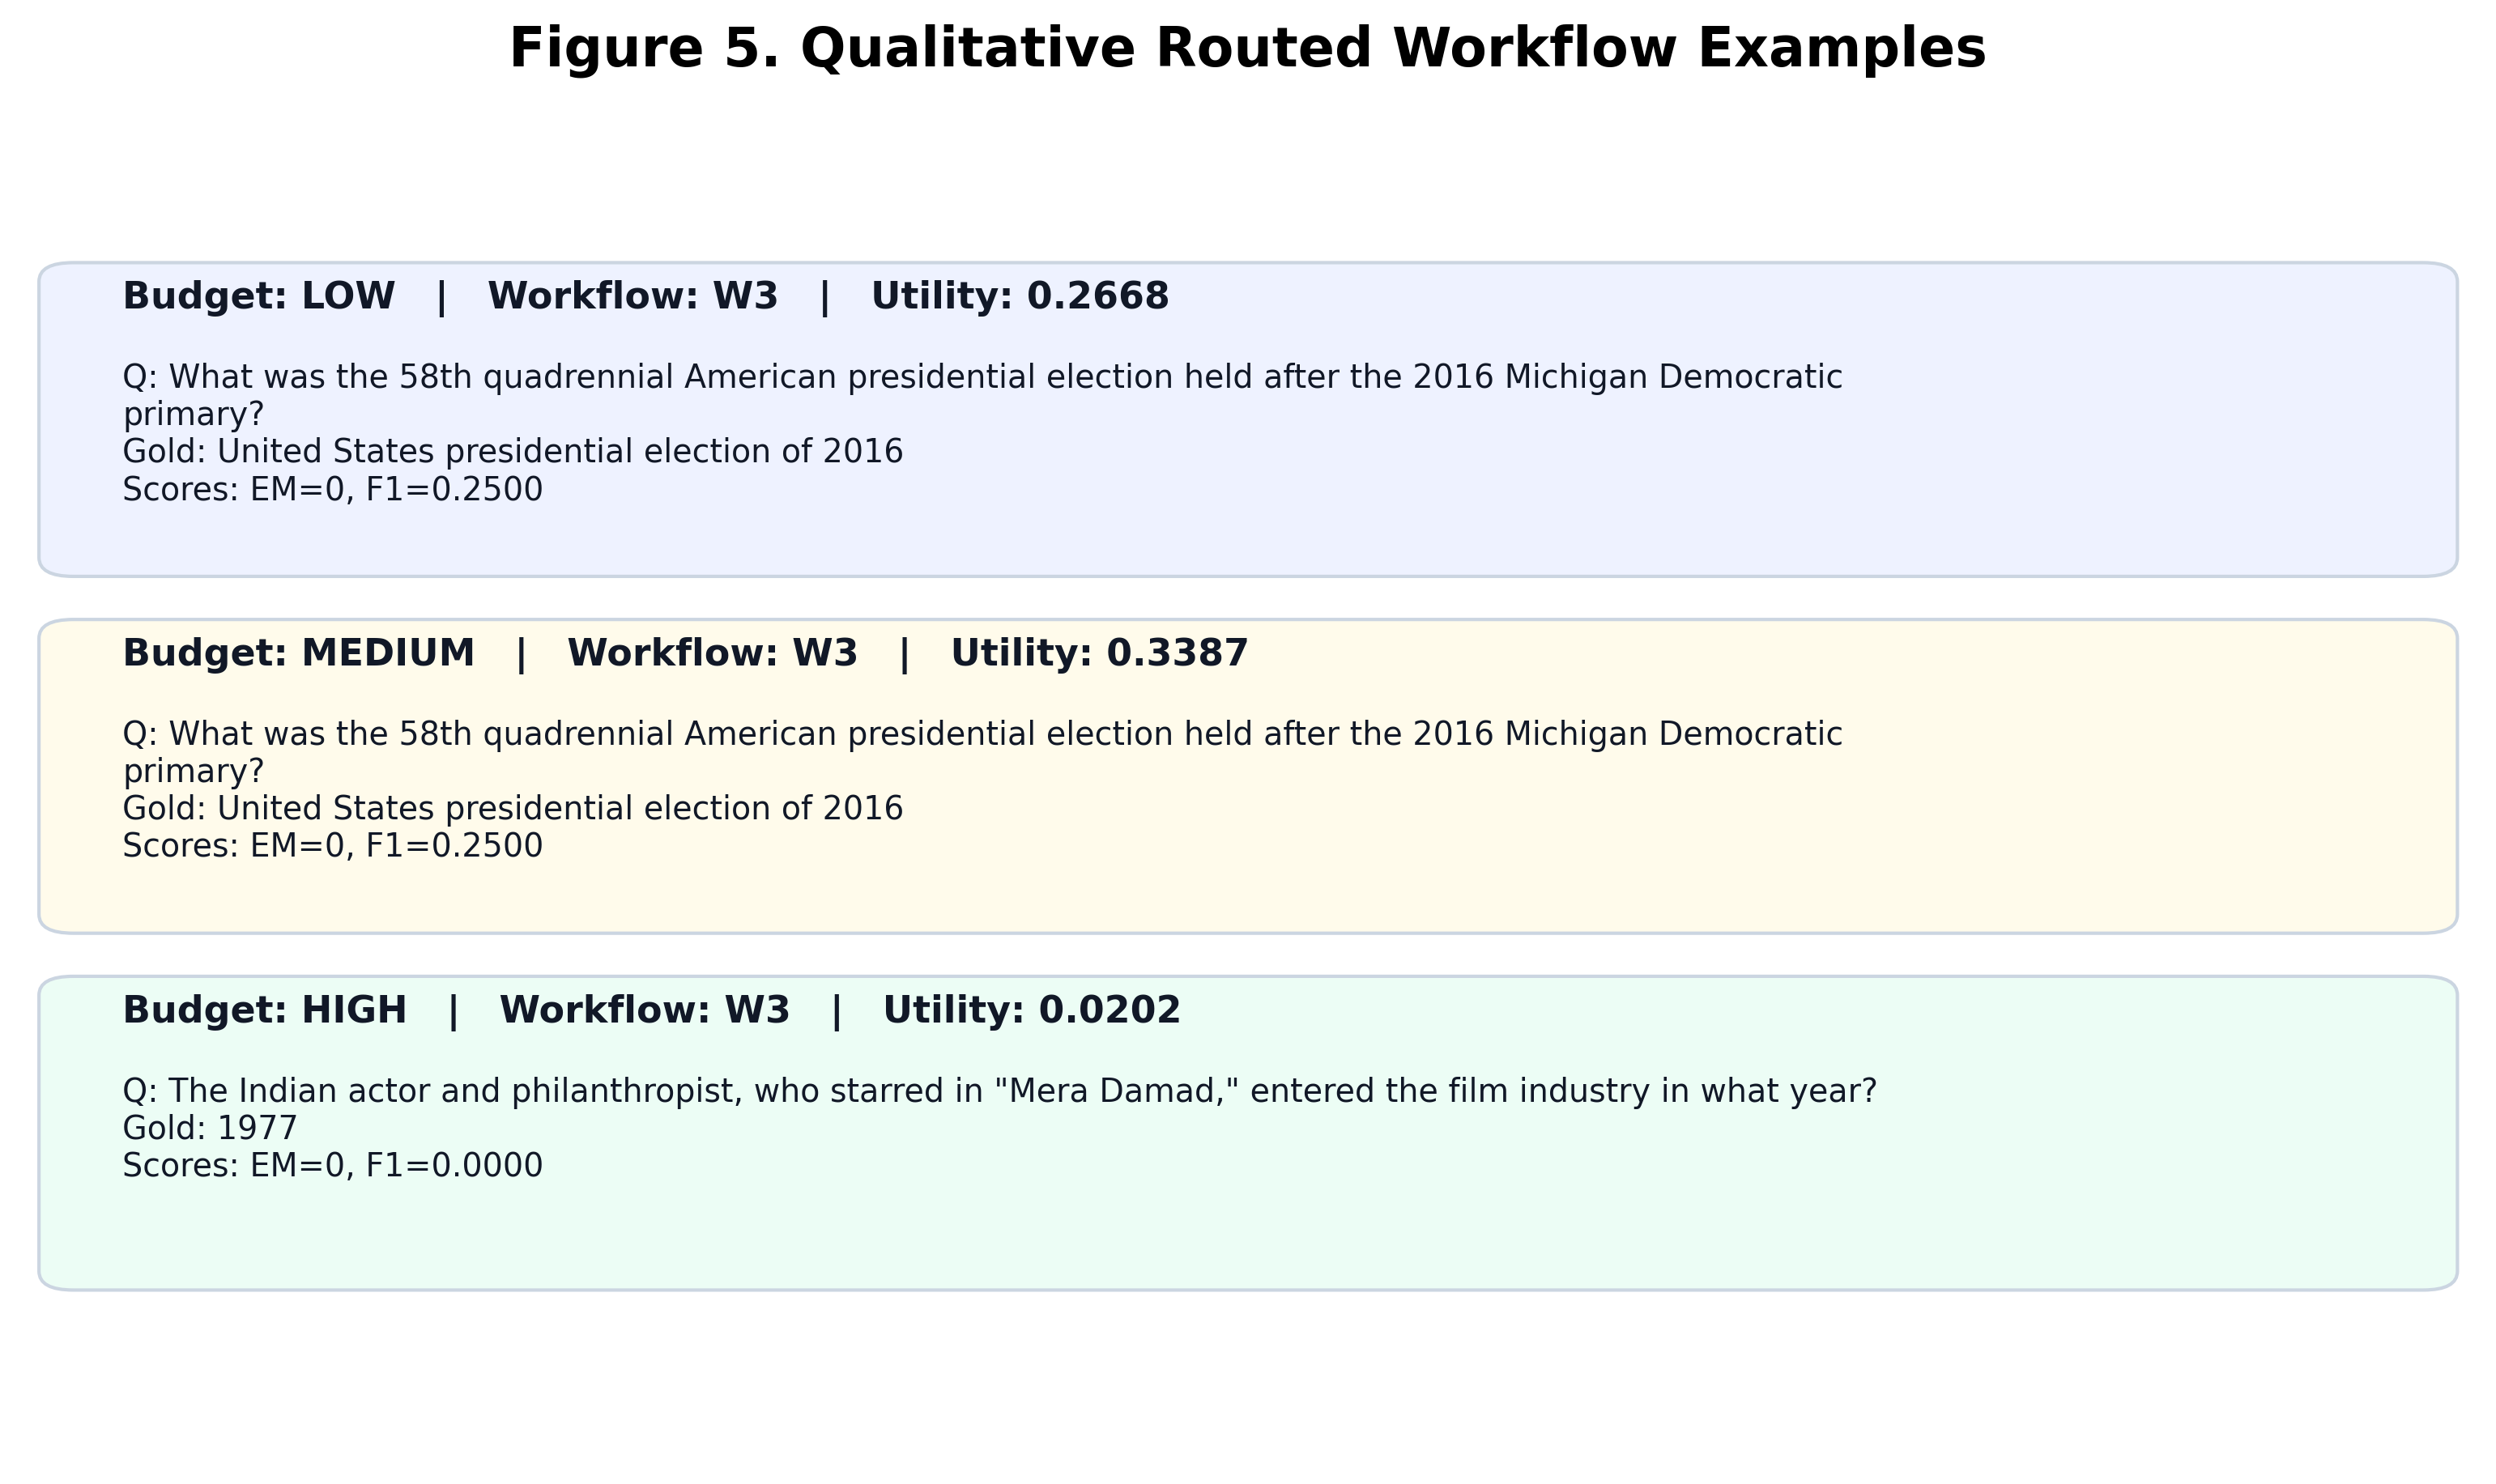
\includegraphics[width=0.92\linewidth]{figures/figure_5_qualitative_examples.png}
\caption{Qualitative examples comparing direct answering, retrieval-based answering, and routed workflow decisions.}
\label{fig:qualitative_results}
\end{figure}
\vnote{Thêm 3 ví dụ định tính: một câu W1 trả lời đúng với chi phí thấp, một câu W3 cần evidence selection, một câu thất bại do retrieve sai hoặc answer hallucination. Nên chụp từ output JSON hoặc Streamlit app.}

\section{Additional Study}

Beyond the main budget-routing evaluation, the project includes an offline full-system reinforcement-learning and promotion framework. This layer is important because adaptive RAG systems can regress when a new policy improves one budget mode but damages another. MAP-RAG-Gym therefore treats policy updates as candidates that must pass evaluation gates before becoming the active bundle. This is a practical engineering adaptation of the reinforcement-learning ideas in MAO-ARAG, where policy optimization is desirable only when it maintains an acceptable cost--quality balance \cite{chen2025maoarag}.

The exported system overview marks online readiness as true and recommends \texttt{online\_full\_system\_rl\_with\_selective\_critic}. The high-budget bandit gate also passes with average regret 0.0352 and exact best-rate 0.8047. These values are important because they measure routing quality relative to an oracle-like best workflow decision. A high best-rate suggests that the router frequently selects the empirically best option, while low regret suggests that even mistakes are not extremely costly.

\subsection{Streamlit Demonstration Application}

In addition to the offline experiments, MAP-RAG-Gym includes a Streamlit application that turns the project into an interactive demonstration system. The purpose of this application is not to replace the quantitative evaluation, but to make the architecture, routing decisions, workflow traces, and exported metrics easier to inspect. The interface is organized as a dashboard with a left sidebar and several analysis tabs. The sidebar summarizes the current system status, including whether online reinforcement-learning readiness is satisfied, the best budget mode, and the workflow library W1--W6. This layout makes the workflow definitions visible while the user navigates across different evaluation views.

The \textit{Overview} tab presents the high-level system state. It shows the utility values for low, medium, and high budget modes as compact metric cards, allowing the user to immediately observe the quality--cost trend reported in the main experiments. It also includes a simplified architecture sketch that separates the macro layer, the micro critic layer, and the system layer. This tab is useful for communicating the main idea of the project: a question and budget mode enter the macro router, a workflow is selected, micro critics can rerank intermediate candidates, and system gates decide whether a policy can be promoted.

The \textit{Architecture} tab is intended to explain the components of MAP-RAG-Gym in more detail. It supports the same story as Figure~\ref{fig:model_architecture}: the macro router performs workflow-level selection, the workflow library executes different RAG strategies, and the process critics evaluate local decisions inside query rewriting, retrieval or selection, and answer generation. The \textit{Experiment Comparison} tab is used to compare dataset--model configurations and exported metrics across runs. It connects directly to the report tables by letting the user inspect how HotpotQA and 2WikiMultihopQA behave under different local LLMs and budgets.

The \textit{Macro Layer} tab focuses on routing behavior. It is designed to show how workflow decisions change across budget modes and configurations. This view is important because the project's main contribution is not only answer generation but adaptive workflow selection. The \textit{Micro Layer} tab focuses on process-critic evaluation, especially QR and AG critics. It helps inspect whether critic scores are reliable enough to support reranking or should remain offline diagnostic signals. The \textit{System Gates} tab summarizes readiness checks such as regret, best-rate, token multiplier, utility gap, and promotion status. This tab operationalizes the safety argument that learned policies and critics should pass non-regression gates before deployment.

The \textit{Visualizations} tab generates and displays the report figures directly from exported metrics, including dataset examples, budget-utility comparison, high-budget bandit cross-validation, and qualitative examples. This reduces the risk of manually drawing figures that do not match the experiment files. Finally, the \textit{Live Demo} tab allows a user to enter a question, select an LLM provider and local model, choose a dataset corpus, set a budget mode, and run the pipeline. The screenshots show an example question about \textit{Pride and Prejudice}; the system selects a fallback W3 workflow, returns the answer \textit{Persuasion}, and displays utility, EM, F1, token count, and step-level pipeline details. This live view is useful for demonstration because it exposes not only the final answer but also the selected workflow and intermediate module scores.

\begin{figure}[H]
\centering
% \includegraphics[width=0.95\linewidth]{figures/streamlit_dashboard_overview.png}
\caption{Streamlit dashboard for MAP-RAG-Gym, including overview metrics, architecture tabs, visualization utilities, system gates, and a live interactive Q\&A demo.}
\label{fig:streamlit_dashboard}
\end{figure}
\vnote{Có thể chụp 2--3 ảnh từ Streamlit app để đưa vào Figure này: Overview tab hiển thị metric cards và architecture sketch; Live Demo tab trước khi chạy pipeline; Live Demo tab sau khi chạy có answer, utility, EM/F1, tokens và pipeline steps. Nếu muốn tiết kiệm trang, ghép ảnh thành một figure nhiều panel (a), (b), (c).}

\begin{table}[H]
\centering
\caption{Contribution-oriented summary of MAP-RAG-Gym.}
\label{tab:contribution_summary}
\begin{tabular}{p{0.26\linewidth}p{0.40\linewidth}p{0.24\linewidth}}
\toprule
\textbf{Contribution} & \textbf{Evidence} & \textbf{Interpretation} \\
\midrule
Budget-aware macro routing & Utility increases from 0.2776 in low mode to 0.4375 in high mode & System exposes controllable quality--cost trade-off. \\
Workflow-level adaptation & Low uses W1/W3; medium uses W1/W2/W3/W6; high uses W2/W3 & Router changes behavior by budget instead of using one fixed pipeline. \\
Process critic training & QR critic Spearman reaches 0.6745 & Query rewrite quality can be ranked with useful reliability. \\
Critic safety analysis & Always-on learned-router critic reduces utility and increases tokens & Critic must be gated rather than blindly enabled. \\
Bandit readiness & Regret 0.0352 and best-rate 0.8047 & High-budget workflow selection is suitable for online-readiness gate. \\
Reproducible reporting & Metrics exported under \texttt{outputs/metrics/} & Report numbers can be traced to project artifacts. \\
\bottomrule
\end{tabular}
\end{table}

\section{Discussion}

The results support the view that adaptive RAG should be evaluated as a system-level decision problem. If the only objective were to maximize answer overlap, the high-budget policy would appear best. However, a real deployment must also consider token usage, retrieval calls, and latency. MAP-RAG-Gym makes these costs visible across two datasets and three models. The low-budget mode gives lower utility but uses fewer tokens and fewer retrieval calls, while the high-budget mode improves answer quality proxies at higher cost. This behavior is aligned with MAO-ARAG's central claim that RAG workflows should be selected dynamically according to query difficulty and cost constraints \cite{chen2025maoarag}.

The cross-dataset comparison reveals that 2WikiMultihopQA is consistently harder than HotpotQA for every model configuration, yielding lower utility, EM, and F1 across all budget modes. This result is consistent with the dataset's design, which includes more diverse and structurally complex reasoning patterns \cite{ho2020twowiki}. The cross-model comparison shows that Llama~3.2 achieves the highest absolute utility on HotpotQA, while Gemma~3 models use more diverse workflow distributions in medium-budget mode, suggesting that larger models may benefit from reflection and rewriting workflows that smaller models cannot leverage as effectively.

The project also shows why process-level supervision is useful but delicate. The QR critic performs well enough to act as an offline reward model across all configurations, which supports the RAG-Gym argument that intermediate actions can be evaluated and optimized \cite{xiong2025raggym}. The Gemma~3 (4B) configuration produces the strongest critic for both QR and AG, suggesting that model consistency may matter more than raw model size for process reward modeling. At the same time, the AG critic and always-on critic deployment results in other configurations reveal that not every critic is immediately suitable for online inference. A weak or misapplied critic can increase token usage and latency without improving utility. Therefore, process critics should be deployed with confidence thresholds, budget constraints, and rollback mechanisms.

Compared with the original MAO-ARAG and RAG-Gym papers, MAP-RAG-Gym is intentionally smaller in scale. It uses locally prepared HotpotQA and 2WikiMultihopQA splits rather than the full original benchmarks, and it uses locally hosted lightweight LLMs via Ollama rather than large-scale fine-tuning. This limitation reduces the strength of claims about generalization. Nevertheless, the project makes a useful contribution at the course-report level because it turns recent research ideas into an inspectable system with five full experimental pipelines: workflow definitions, rollout data, routers, critics, promotion checks, and exported metrics are all present in the repository.

Several limitations remain. First, the evaluation set contains only 90 held-out questions per budget mode, so confidence intervals would be useful in future work. Second, W4 and W5 are included in the workflow library but are not central in the reported final routing distribution; additional experiments should test whether decomposition workflows become more valuable on harder datasets such as Bamboogle \cite{press2022bamboogle}. Third, the AG critic is reliable only in the Gemma~3 (4B) configuration and needs improvement in others. Fourth, online RL is marked ready by gates in some configurations, but actual long-running online policy updates and A/B testing remain future work.

\section{Conclusion}

This report presented MAP-RAG-Gym, a budget-aware adaptive RAG system that combines macro workflow routing inspired by MAO-ARAG with micro process criticism inspired by RAG-Gym. The system implements a workflow library, routers, bandit selection, process critics, evaluation scripts, exported metrics, and readiness gates. Across two multi-hop QA datasets (HotpotQA and 2WikiMultihopQA) and three locally hosted LLMs (Llama~3.2, Gemma~3 12B, and Gemma~3 4B), the system demonstrates consistent budget-performance patterns: utility increases with budget while token cost and latency also grow. On HotpotQA with Llama~3.2, utility ranges from 0.2776 (low budget) to 0.4375 (high budget). On 2WikiMultihopQA, utility is lower across the board, confirming the dataset's greater difficulty. The QR critic achieves strong rank correlation (up to Spearman~0.7701 with Gemma~3 4B), while the AG critic is usable only in specific model configurations. The cross-model, cross-dataset design provides evidence that adaptive RAG routing is robust to model choice, though absolute quality varies. Overall, the project demonstrates that adaptive RAG can be studied not only as answer generation, but as a controllable system that chooses workflows, evaluates intermediate decisions, and balances quality against cost across different deployment conditions. Future work should expand to additional benchmarks, improve the AG critic, test decomposition workflows, and run actual online RL with A/B testing and non-regression safeguards.

\section*{Checklist Before Submission}
\addcontentsline{toc}{section}{Checklist Before Submission}

Before submitting the final PDF, the student should update all identity fields on the cover page and contribution table. The student should also add at least three figures: the MAP-RAG-Gym architecture diagram, a budget utility chart, and qualitative examples from actual output files or the Streamlit application. Finally, all numeric claims should be checked against the latest CSV exports if experiments are rerun.

\section*{References}
\addcontentsline{toc}{section}{References}

\begin{thebibliography}{99}

\bibitem{chen2025maoarag}
Y. Chen, E. Zhang, L. Yan, S. Wang, J. Huang, D. Yin, and J. Mao, ``MAO-ARAG: Multi-Agent Orchestration for Adaptive Retrieval-Augmented Generation,'' arXiv preprint, 2025.

\bibitem{xiong2025raggym}
G. Xiong, Q. Jin, X. Wang, Y. Fang, H. Liu, Y. Yang, F. Chen, Z. Song, D. Wang, M. Zhang, Z. Lu, and A. Zhang, ``RAG-Gym: Systematic Optimization of Language Agents for Retrieval-Augmented Generation,'' arXiv preprint, 2025.

\bibitem{lewis2020rag}
P. Lewis, E. Perez, A. Piktus, F. Petroni, V. Karpukhin, N. Goyal, H. Kuttler, M. Lewis, W. Yih, T. Rocktaschel, S. Riedel, and D. Kiela, ``Retrieval-Augmented Generation for Knowledge-Intensive NLP Tasks,'' in \textit{Advances in Neural Information Processing Systems}, 2020.

\bibitem{karpukhin2020dpr}
V. Karpukhin, B. Oguz, S. Min, P. Lewis, L. Wu, S. Edunov, D. Chen, and W. Yih, ``Dense Passage Retrieval for Open-Domain Question Answering,'' in \textit{Proceedings of EMNLP}, 2020, pp. 6769--6781.

\bibitem{yang2018hotpotqa}
Z. Yang, P. Qi, S. Zhang, Y. Bengio, W. Cohen, R. Salakhutdinov, and C. D. Manning, ``HotpotQA: A Dataset for Diverse, Explainable Multi-hop Question Answering,'' in \textit{Proceedings of EMNLP}, 2018, pp. 2369--2380.

\bibitem{ho2020twowiki}
X. Ho, A.-K. D. Nguyen, S. Sugawara, and A. Aizawa, ``Constructing a Multi-hop QA Dataset for Comprehensive Evaluation of Reasoning Steps,'' arXiv preprint arXiv:2011.01060, 2020.

\bibitem{press2022bamboogle}
O. Press, M. Zhang, S. Min, L. Schmidt, N. A. Smith, and M. Lewis, ``Measuring and Narrowing the Compositionality Gap in Language Models,'' arXiv preprint arXiv:2210.03350, 2022.

\bibitem{yao2023react}
S. Yao, J. Zhao, D. Yu, N. Du, I. Shafran, K. Narasimhan, and Y. Cao, ``ReAct: Synergizing Reasoning and Acting in Language Models,'' in \textit{International Conference on Learning Representations}, 2023.

\bibitem{asai2023selfrag}
A. Asai, Z. Wu, Y. Wang, A. Sil, and H. Hajishirzi, ``Self-RAG: Learning to Retrieve, Generate, and Critique through Self-Reflection,'' arXiv preprint arXiv:2310.11511, 2023.

\bibitem{li2025searcho1}
X. Li, G. Dong, J. Jin, Y. Zhang, Y. Zhou, Y. Zhu, P. Zhang, and Z. Dou, ``Search-o1: Agentic Search-Enhanced Large Reasoning Models,'' arXiv preprint arXiv:2501.05366, 2025.

\bibitem{jin2025searchr1}
B. Jin, H. Zeng, Z. Yue, J. Yoon, S. Arik, D. Wang, H. Zamani, and J. Han, ``Search-R1: Training LLMs to Reason and Leverage Search Engines with Reinforcement Learning,'' arXiv preprint arXiv:2503.09516, 2025.

\bibitem{schulman2017ppo}
J. Schulman, F. Wolski, P. Dhariwal, A. Radford, and O. Klimov, ``Proximal Policy Optimization Algorithms,'' arXiv preprint arXiv:1707.06347, 2017.

\bibitem{rafailov2023dpo}
R. Rafailov, A. Sharma, E. Mitchell, S. Ermon, C. D. Manning, and C. Finn, ``Direct Preference Optimization: Your Language Model is Secretly a Reward Model,'' in \textit{Advances in Neural Information Processing Systems}, 2023.

\bibitem{robertson1994bm25}
S. E. Robertson and S. Walker, ``Some Simple Effective Approximations to the 2-Poisson Model for Probabilistic Weighted Retrieval,'' in \textit{Proceedings of SIGIR}, 1994, pp. 232--241.

\end{thebibliography}

\end{document}
